\documentclass[border=10pt]{standalone}
\usepackage{tkz-fct}
\usepackage{tkz-base}
\usepackage{array}

\begin{document}

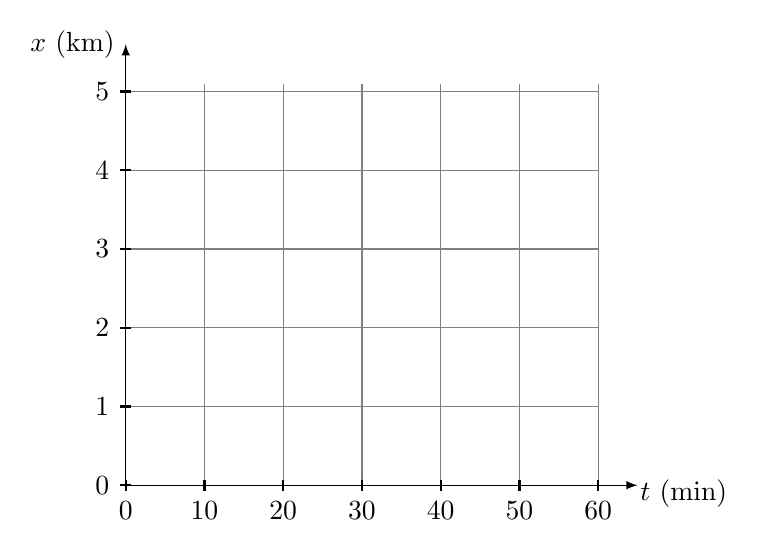
\begin{tikzpicture}
% Tableau en LaTeX standard avec tkz-text

% Repère quadrillé
\tkzInit[xmin=0,xmax=60,xstep=10,ymin=0,ymax=5.1, ystep=1]
\tkzGrid
\tkzDrawX[label = $t$ (min), right]
\tkzDrawY[label = $x$ (km)]
\tkzLabelXY
\tkzFct[line width=2pt, domain=0:10]{(1/10.)*\x +1}
\tkzFct[line width=2pt, domain=10:30]{(3/20.)*(\x-10) +2}
\tkzFct[line width=2pt, domain=30:40]{5}
\tkzFct[line width=2pt, domain=40:50]{(-4/10.)*(\x-40) +5}
\tkzFct[line width=2pt, domain=50:60]{(-1/10.)*(\x-50) +1}

\end{tikzpicture}

\end{document}
